\documentclass{slide}

\usepackage{changepage}
\usepackage{tikz}
%\usepackage{pgfpages}
%\setbeameroption{show notes on second screen}

\title{Decomposing Monoliths}
\subtitle{CSSE6400}
\author{Richard Thomas}
\date{\week{12}}
\titlegraphic {
    \begin{tikzpicture}[overlay,remember picture]
    \node[left=0.1cm] at (current page.-9){
        \includegraphics[width=7cm]{images/decomposing\_computer.png}
    };
    \end{tikzpicture}
}

\begin{document}

\maketitle

\questionanswer{What are the benefits of a monolith architecture?}{
    \begin{itemize}[<+(1)->]
        \item Simple deployment
        \item Simple communication between modules
        \item Simple system testing \& debugging
    \end{itemize}
}

\questionanswer{Why do monoliths have a bad name?}{
    \begin{itemize}[<+(1)->]
        \item Many legacy system nightmares were monoliths
        \item Easy to defeat modularity
        \item Cannot scale components of system
        \item Monolith databases scale poorly
    \end{itemize}
}

\questionanswer{What can be done if a monolith architecture is no longer suitable?}{
    \begin{itemize}[<+(1)->]
        \item Greenfields replacement
        \note<2>{Replacement
					 \begin{itemize}
        			     \item Pro: Can choose any suitable architecture.
        				 \item Risk: Developing a new system and maintaining existing.
        			 \end{itemize}
        			}
        \item Migrate to another architecture
        \note<3>{Migration
					 \begin{itemize}
        			     \item Adaptive maintenance, changing architecture slowly.
        				 \item Some limitation on choice of architecture, but most sophisticated architectures can be used.
        			 \end{itemize}
        			}
    \end{itemize}
}

\questionanswer{How do I migrate a monolith to a new architecture?}{Decompose the monolith into services.}
\note{Implies a service-based or microservices architecture.}

\begin{frame}{Strangler Fig Pattern}
    \vspace{1pt}
    \begin{columns}
    \column{0.65\textwidth}
      {\LARGE
        \begin{itemize}
            \item Develop API for application's UI
            \vspace{1mm}
            \item Proxy intercepts API calls
            \begin{itemize}
                \Large\item Proxy directs calls to application or new services
            \end{itemize}
            \vspace{1mm}
            \item Implement a service
            \begin{itemize}
                \Large\item Redirect calls to service
            \end{itemize}
            \item Progressively replace monolith
            \item Shadow \& Blue-Green Deployment
        \end{itemize}
      }
    \column{0.35\textwidth}
        \centering
        
\includegraphics[height=0.9\textheight]{images/strangler-fig.jpg}
    \end{columns}
\end{frame}
\note[itemize]{
    \item May already have an API if the UI is a web or mobile app.
    \item Initially deploy proxy and new interface into production, with only existing monolith. Test it works as expected.
    \item Shadow deployment to test service with application.
    \item Blue-Green deployment to switch over to using service.
}

\begin{frame}{Monolith Deployment}
    \begin{adjustwidth}{-12mm}{-12mm}
        \centering
        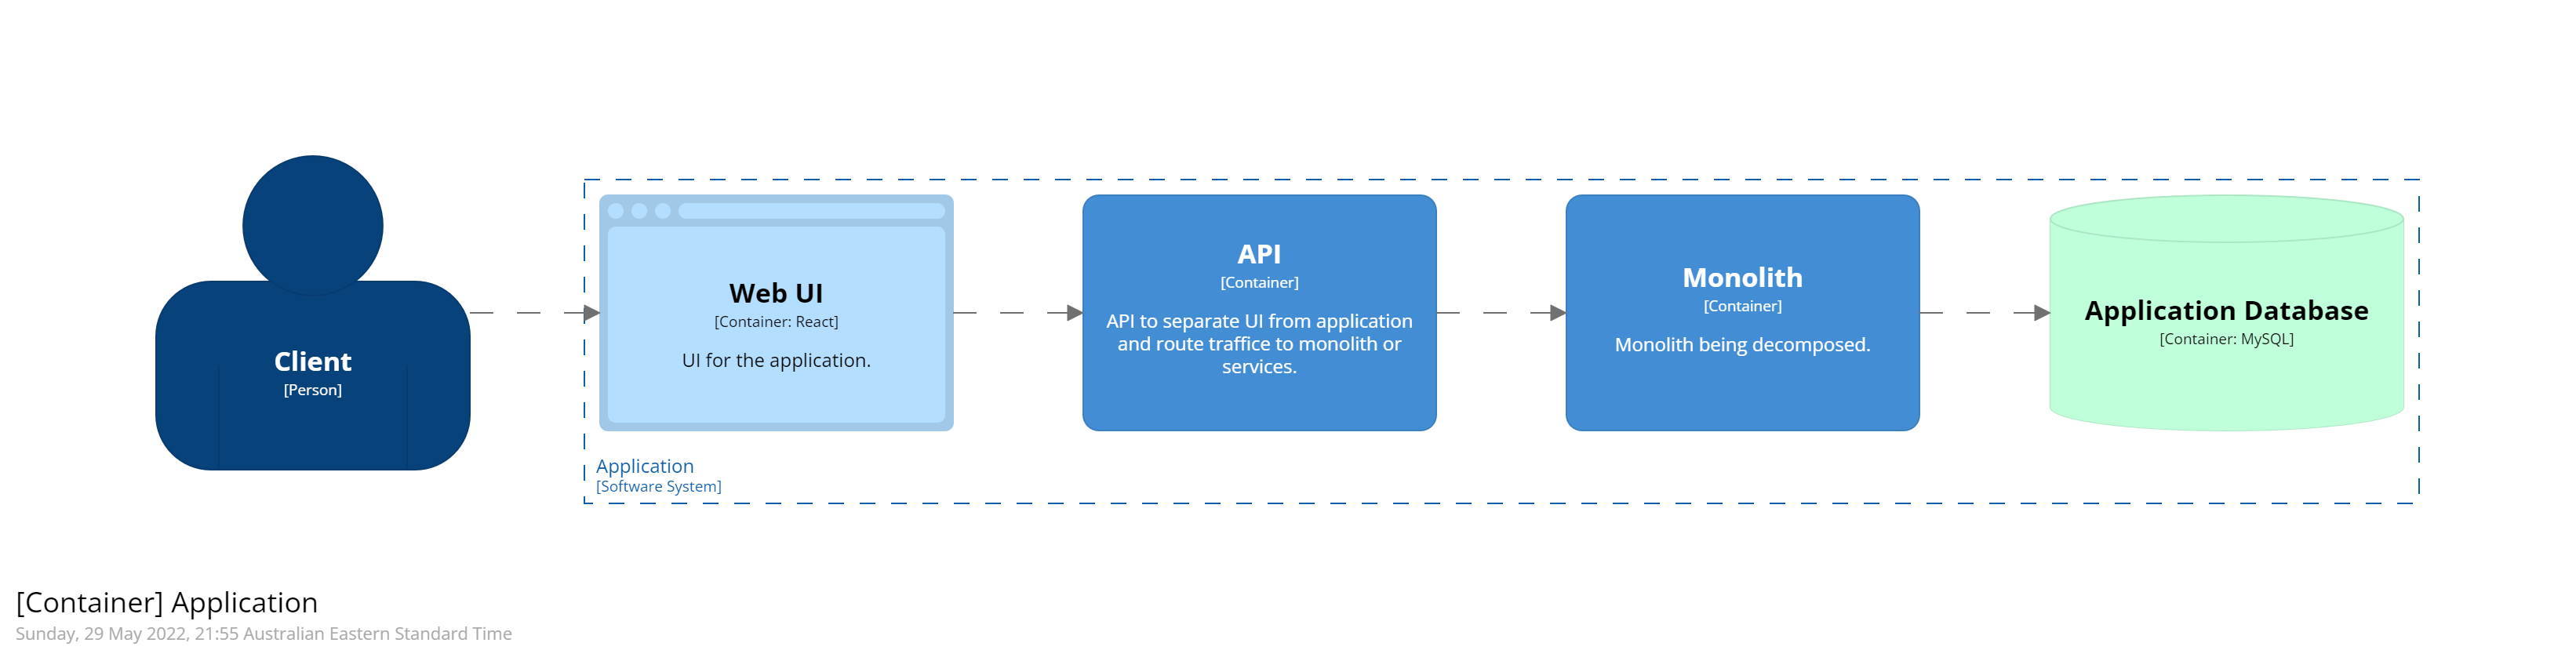
\includegraphics[trim=195 195 195 195,clip,width=0.97\paperwidth]{diagrams/decompose1.png}
    \end{adjustwidth}
\end{frame}

\begin{frame}{Monolith Decompose: Step 1}
    \begin{adjustwidth}{-12mm}{-12mm}
        \centering
        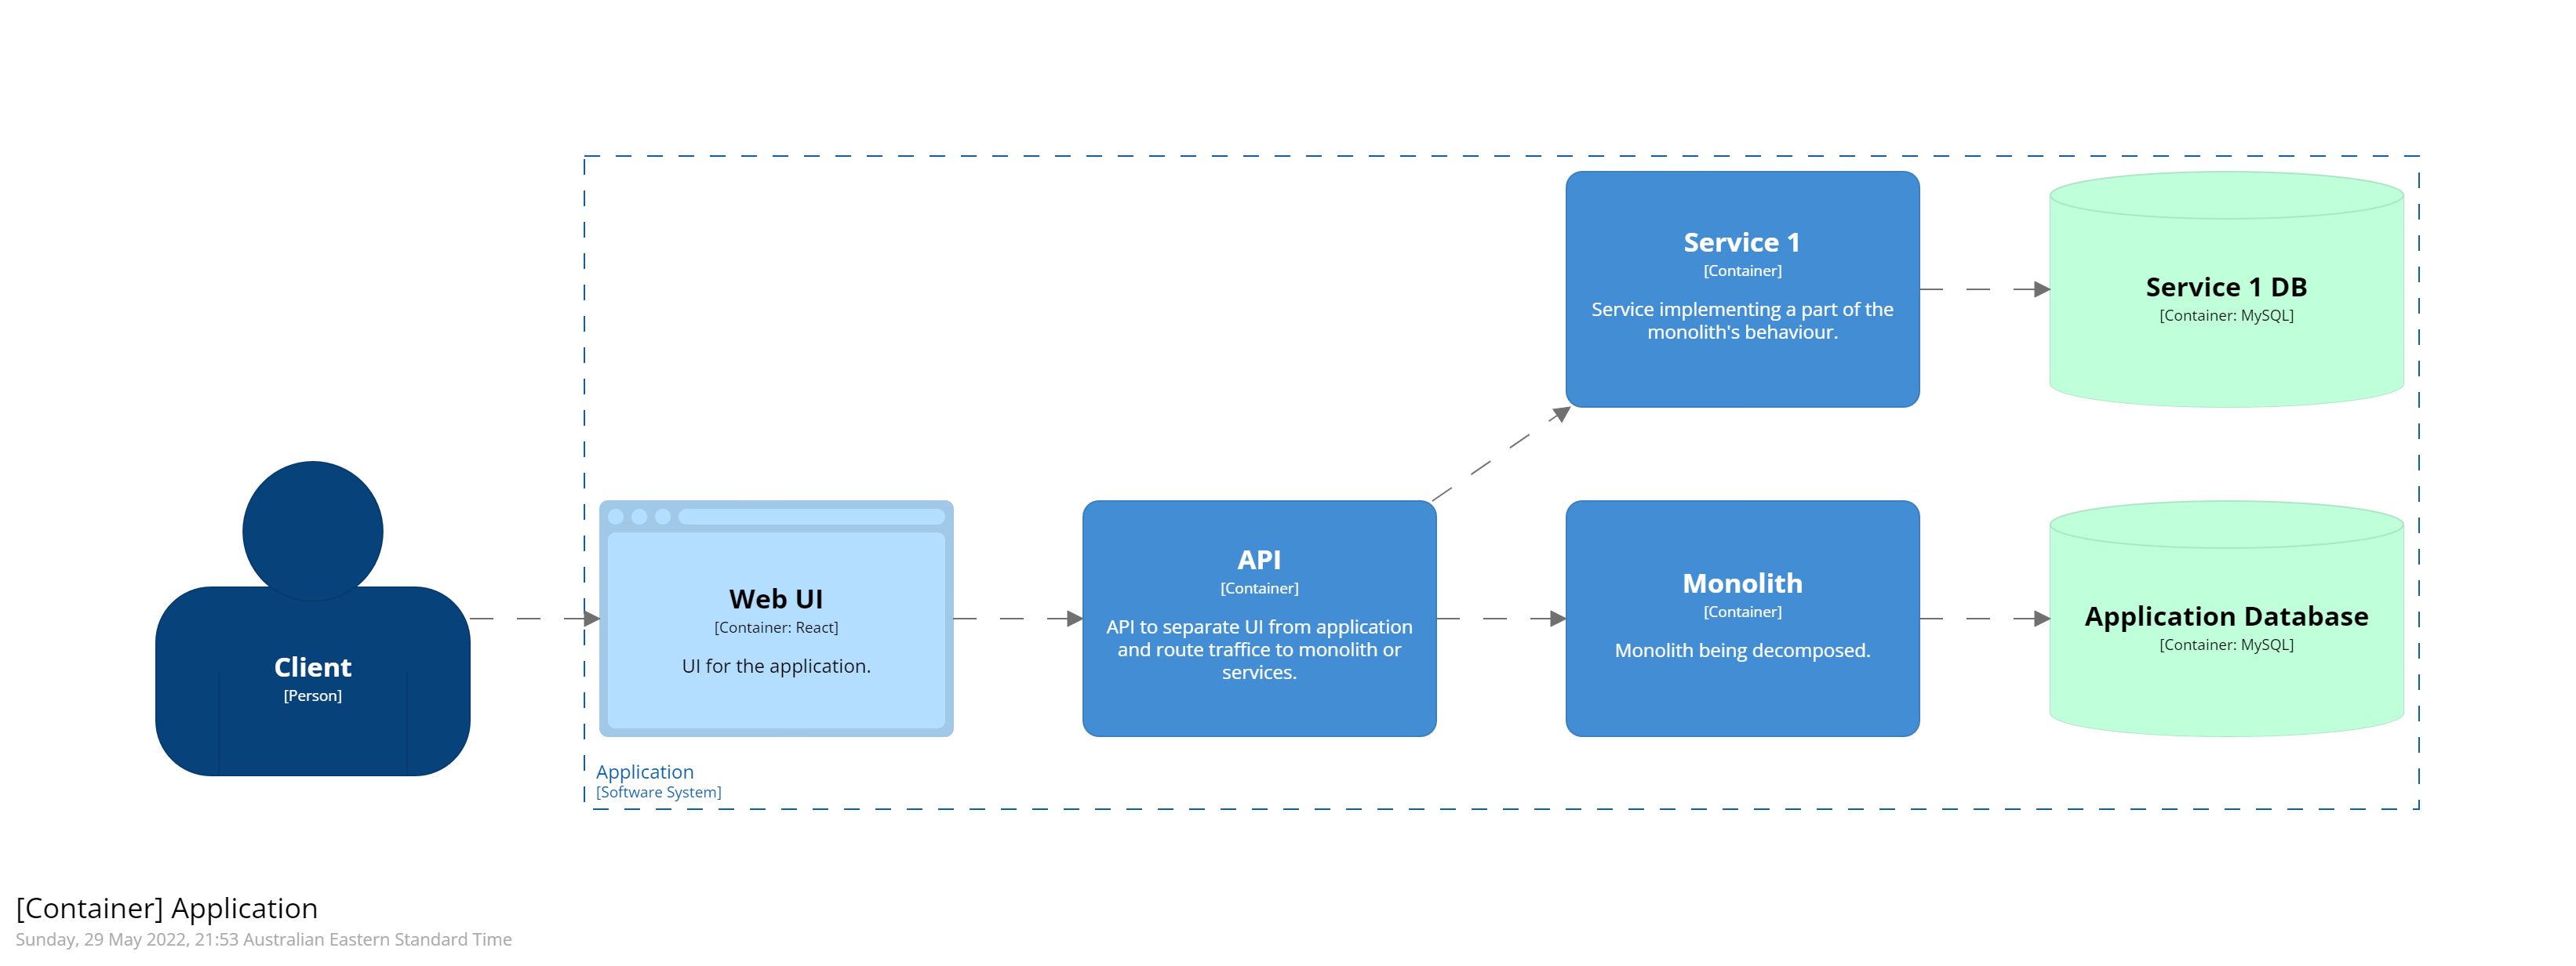
\includegraphics[trim=195 195 195 195,clip,width=0.97\paperwidth]{diagrams/decompose2.png}
    \end{adjustwidth}
\end{frame}

\begin{frame}{Monolith Decompose: Step 2}
    \begin{adjustwidth}{-12mm}{-12mm}
        \centering
        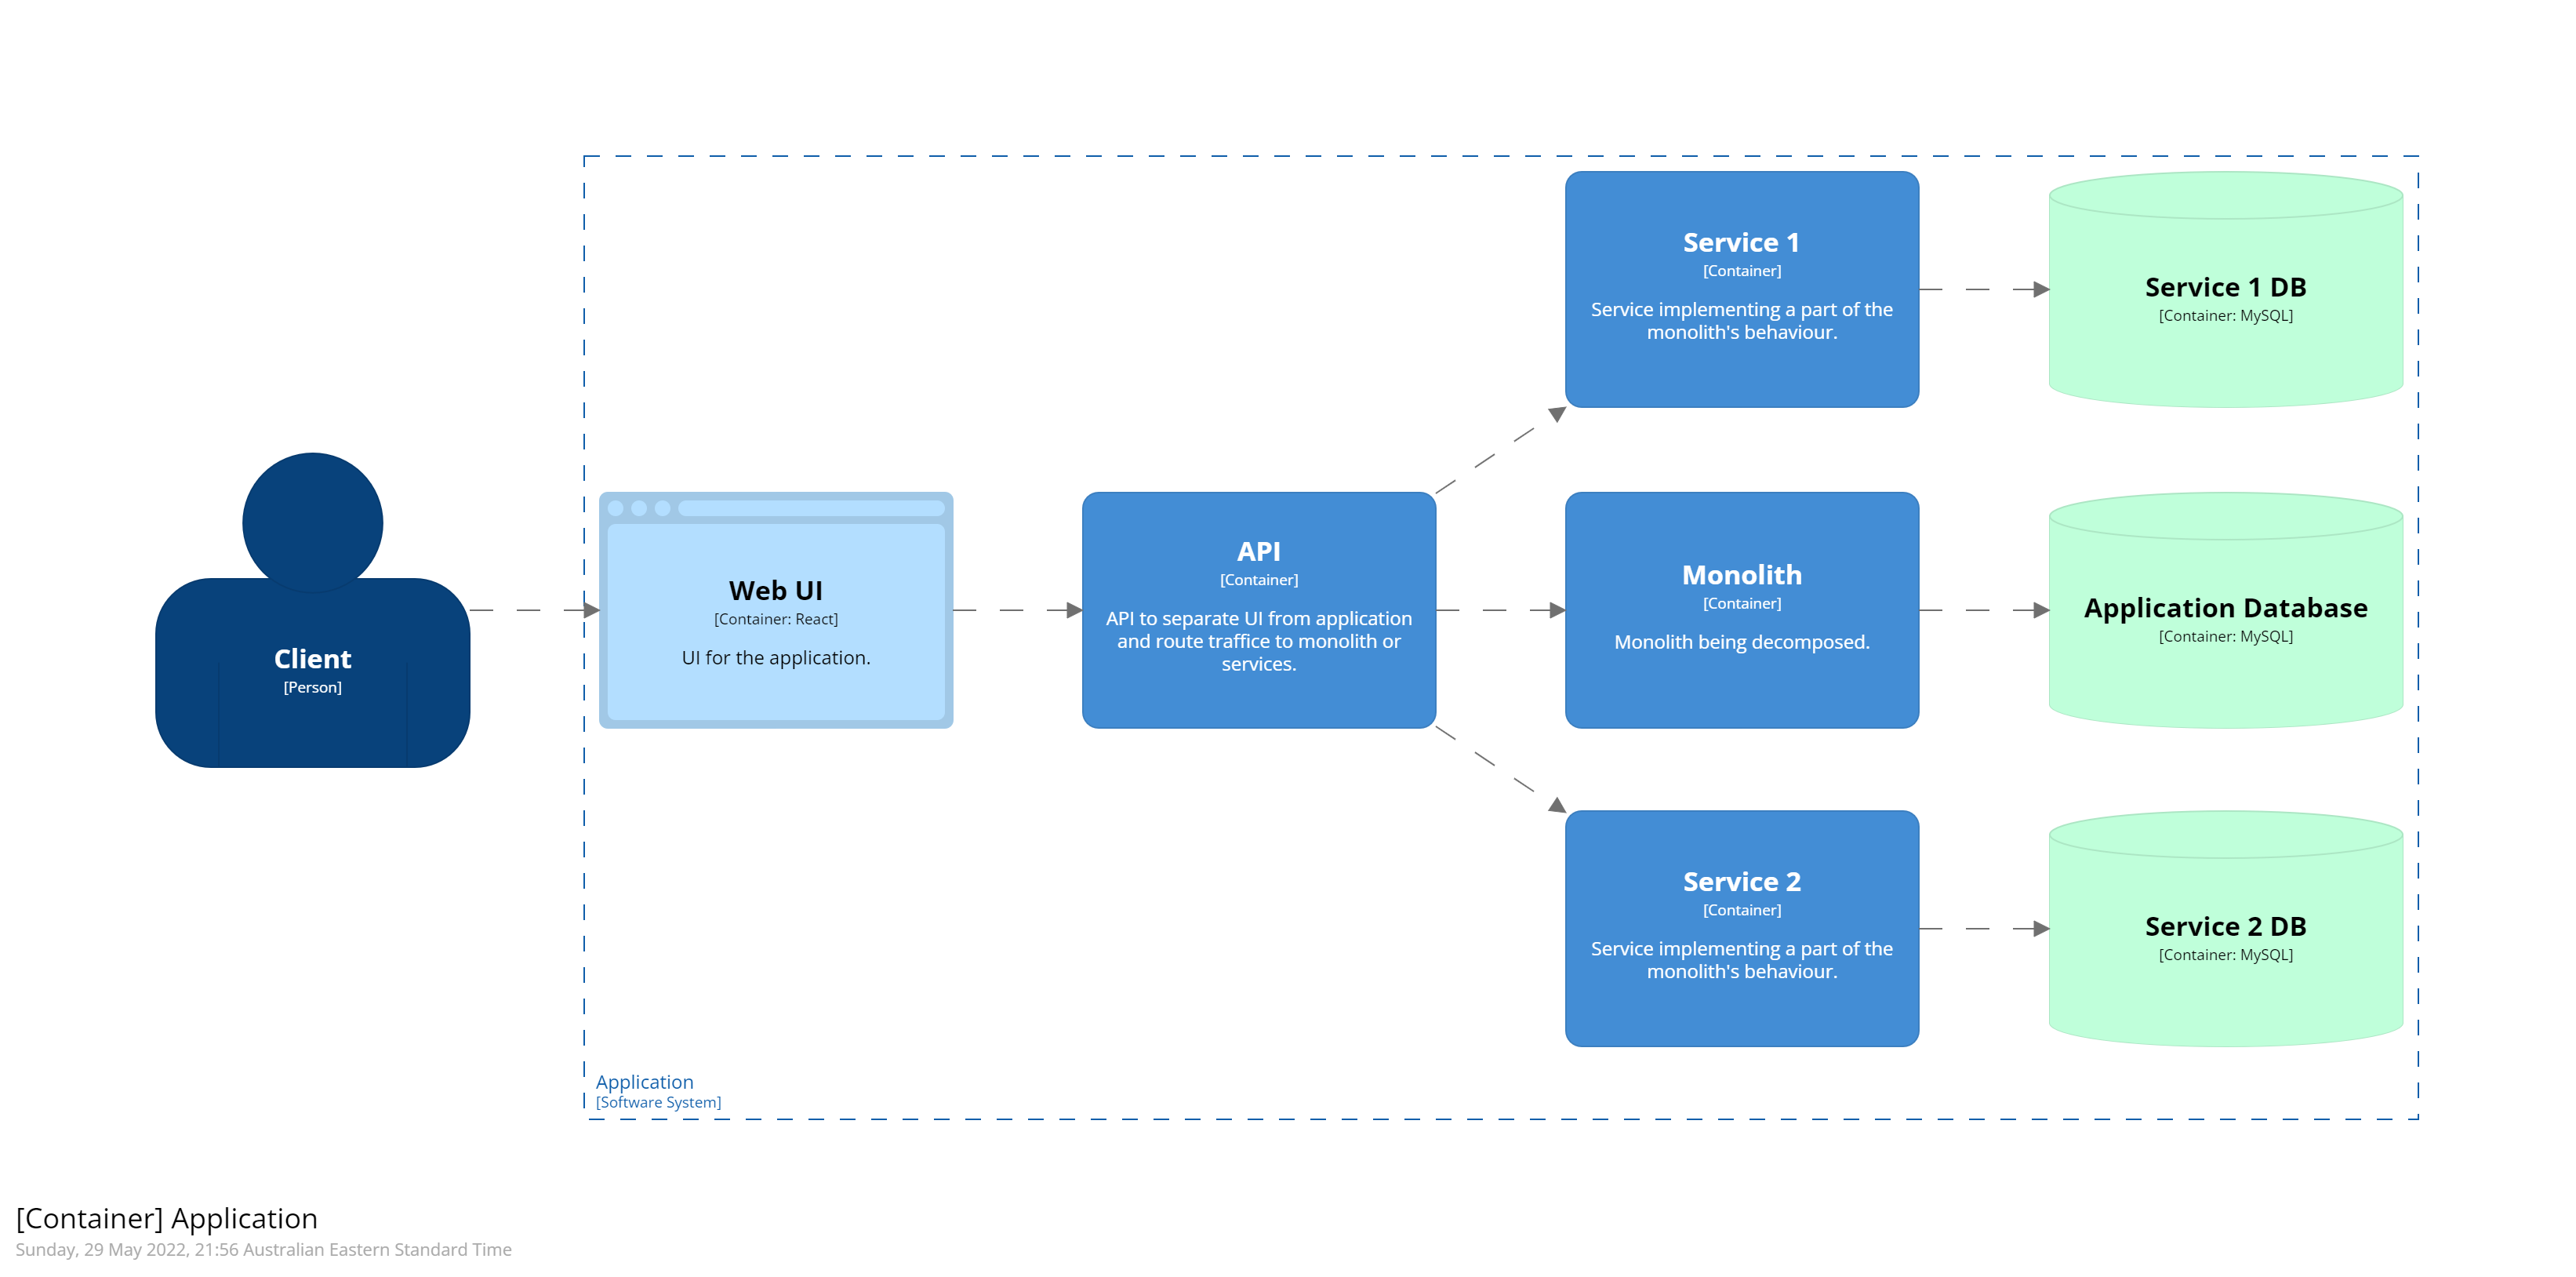
\includegraphics[trim=195 195 195 195,clip,width=0.97\paperwidth]{diagrams/decompose3.png}
    \end{adjustwidth}
\end{frame}

\begin{frame}{Decomposition Process}
\vspace{1pt}
{\huge
\begin{itemize}
    \item Identify bounded-contexts
    \vspace{3mm}
    \item Simple first service
    \begin{itemize}
        \LARGE\item e.g. Authentication
    \end{itemize}
    \vspace{3mm}
    \item Minimise dependency from services to monolith
    \begin{itemize}
        \LARGE\item Monolith may use services
    \end{itemize}
\end{itemize}
}
\end{frame}
\note[itemize]{
    \item Use first service (or first few) to validate approach and deployment infrastructure.
    \item Minimise changes required in monolith.
}

\begin{frame}{Decomposition Process}
\vspace{1pt}
{\huge
\begin{itemize}
    \item Reduce coupling between bounded-contexts
    \vspace{1mm}
    \begin{itemize}
        \LARGE\item e.g. Customer account management
        \begin{itemize}
            \Large\item Profile, Wish List, Payment Preferences -- separate services
        \end{itemize}
    \end{itemize}
    \vspace{3mm}
    \item Decouple vertically
    \vspace{1mm}
    \begin{itemize}
        \LARGE\item Service delivers entire bounded-context
        \begin{itemize}
            \Large\item Data is decoupled from monolith
        \end{itemize}
    \end{itemize}
\end{itemize}
}
\end{frame}
\note[itemize]{
    \item Account management may be tightly coupled in monolith. Separate each aspect (context), one at a time.
    \item Do not focus only on UI or internal components, service needs to implement all parts of the business process.
    \item Data management needs to be decentralised.
}

\begin{frame}{Decomposition Process}
\vspace{1pt}
{\huge
\begin{itemize}
    \item Focus on pain points
    \begin{itemize}
        \LARGE\item Bottlenecks
        \LARGE\item Frequently changing behaviour
    \end{itemize}
    \vspace{3mm}
    \item Rewrite, don't reuse
    \begin{itemize}
        \LARGE\item Redesign for new infrastructure
        \vspace{2mm}
        \LARGE\item Reuse complex logic
        \vspace{-1mm}
        \begin{itemize}
            \Large\item e.g. Discounts based on customer loyalty and behaviour, bundle offers, \dots
        \end{itemize}
    \end{itemize}
\end{itemize}
}
\end{frame}
\note[itemize]{
    \item Extract services that deliver highest value.
    \item What contexts may need to scale more than others?
    \item What contexts change more frequently and benefit from separate deployment?
    \item Services deliver capabilities provided by monolith.
    \item Most often it is better to rewrite the capability to take advantage of new infrastructure.
    \item Only reuse code that has complex logic that will be difficult to duplicate and test fully.
}

\begin{frame}{Atomic Decomposition}
\vspace{1pt}
{\huge
\begin{itemize}
    \item Refactor monolith
    \vspace{2mm}
    \begin{itemize}
        \LARGE\item Use service to deliver application functionality
        \begin{itemize}
            \Large\item Monolith may need to invoke service
        \end{itemize}
        \vspace{-1mm}
        \LARGE\item Remove service logic from monolith
    \end{itemize}
\end{itemize}
}
\end{frame}
\note[itemize]{
    \item Atomic replacement of monolith behaviour by service's behaviour.
    \item Don't deploy production code with service behaviour left in monolith.
            Leads to a maintenance nightmare determining where behaviour is used, or it may be used in both the monolith and service.
}

\point[Stepwise Decomposition]{Replace application functionality one service at a time.}

\definition{Macroservice}{Separate service, but may span more than one domain or share a database with the monolith or other services.}
\note[itemize]{
    \item Similar scalability and deployment issues to a monolith, but grouped by clusters of macroservices if they share a database.
    \item Interim step to build microservices.
}

\definition{Nanoservice}{Service that depends on other services and cannot be deployed independently -- its context is too small.}
\note[itemize]{
    \item Anti-pattern where services are too fine grained and need to be coupled to deliver business processes.
    \item Some use the term ``nanoservice'' to refer to independently deployable functions, similar to serverless architecture.
}

\end{document}